% DESCRIPTION: This file presents the research findings, discussion, implications, and limitations of the study.
\section{Results and Discussion}
\textbf{Results:} Present findings clearly.\\
\textbf{Discussion:} Discuss the findings.\\
\textbf{Implications:} Describe implications.\\
\textbf{Research contribution:} State contributions.\\
\textbf{Limitations:} Mention limitations.\\
\textbf{Suggestions:} Provide suggestions.

\begin{table}[h]
\centering
\caption{The sample of table format (Center, Cambria, 11)}
\vspace{0.2cm}
\begin{tabular}{|c|l|l|}
\hline
\textbf{No} & \textbf{Description} & \textbf{Explanation} \\
\hline
1 & Description 1 & Explanation \\
\hline
2 & Description 2 & Explanation \\
\hline
3 & Description 3 & Explanation \\
\hline
4 & Description 4 & Explanation \\
\hline
5 & Description 5 & Explanation \\
\hline
\end{tabular}
\end{table}

\begin{figure}[h]
\centering
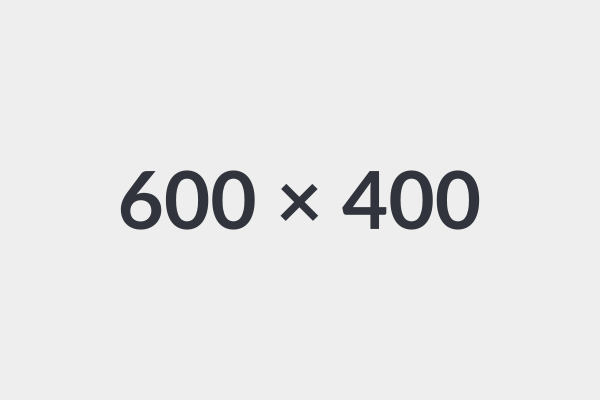
\includegraphics[width=0.6\textwidth]{workspace/assets/images/600x400.png}
\caption{The example of an image of the spectrum absorption coefficients of organic semiconductor materials}
\end{figure}
